% Page 035 — page imprimée 31
% Contenu seul : le préambule et la pagination sont gérés par meyrueis.tex

\begin{center}
{\large\bfseries LES CHAPELIERS DE MEYRUEIS}
\end{center}

\vspace{5em}

Le chapeau fabriqué à Meyrueis était un feutre de laine teint en
noir, à larges bords le plus souvent souples. Tantôt sa coiffe
était ronde, en feutre mou mais résistant, tantôt elle avait
l’allure d’un cône évasé relativement haut.

On distingue deux catégories de chapeaux :

Le feutre souple à larges bords, fabriqué manuellement
protégeant avantageusement le front, le cou et le visage (N° 2,
3, 4, 5 et 6), traditionnellement porté pour les travaux des
champs.

La deuxième catégorie (1, 7, et 8) concerne une seconde
génération de chapeaux plus spécialement confectionnés
pendant la période de mécanisation des ateliers : un galon de
même couleur que le feutre ajoute une note d’élégance... C’est
le chapeau Couderc de 1910, Un secret de fabrication, breveté
le rendait imperméable.

\begin{center}
\textit{(D’après un article de Jean Claude Crespin)}
\end{center}

\begin{center}
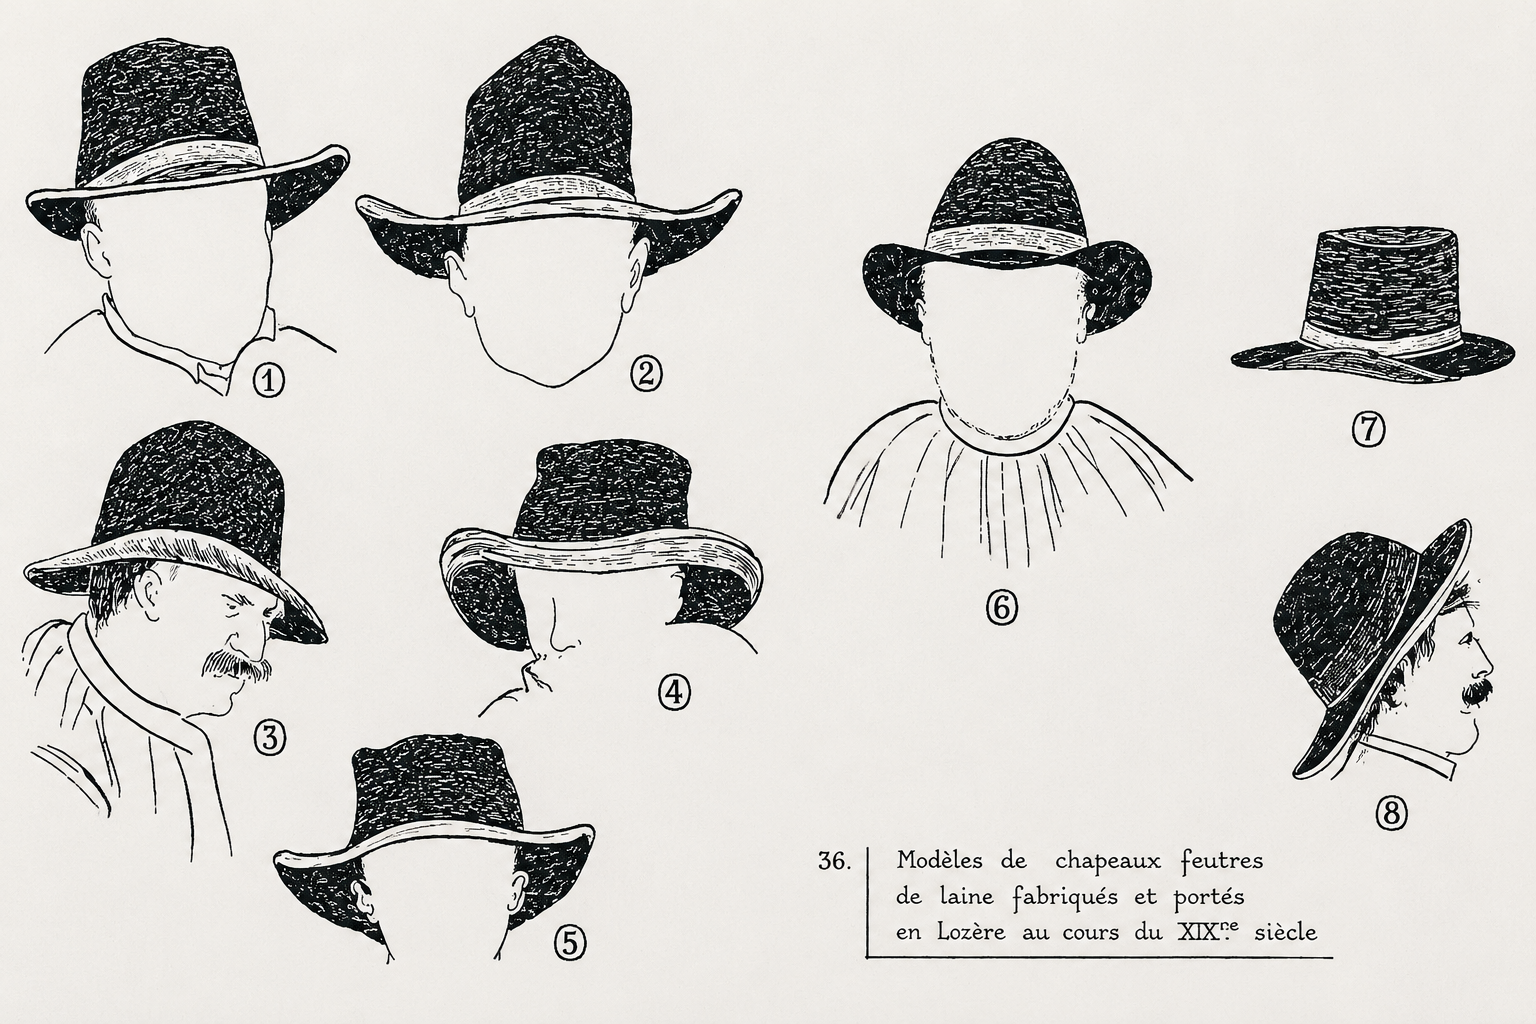
\includegraphics[width=\textwidth]{imgs/035.png}
\end{center}
